\subsection{ FC -51: InfraRed Sensor}
Infrared technology addresses a wide variety of wireless applications. The main areas are sensing and remote controls. In the electromagnetic spectrum, the infrared portion is divided into three regions: near infrared region, mid infrared region and far infrared region.\\
The frequency range of infrared is higher than microwave and lesser than visible light.\\
For optical sensing and optical communication, photo optics technologies are used in the near infrared region as the light is less complex than RF when implemented as a source of signal. Optical wireless communication is done with IR data transmission for short range applications.\\
An infrared sensor emits and/or detects infrared radiation to sense its surroundings.\\
The working of any Infrared sensor is governed by three laws: Planck’s Radiation law, Stephen – Boltzmann law and Wien’s Displacement law.\\
Planck’s law states that “every object emits radiation at a temperature not equal to 00K”. Stephen – Boltzmann law states that “at all wavelengths, the total energy emitted by a black body is proportional to the fourth power of the absolute temperature”. According to Wien’s Displacement law, “the radiation curve of a black body for different temperatures will reach its peak at a wavelength inversely proportional to the temperature”.\\
The basic concept of an Infrared Sensor which is used as Obstacle detector is to transmit an infrared signal, this infrared signal bounces from the surface of an object and the signal is received at the infrared receiver.\\
There are five basic elements used in a typical infrared detection system: an infrared source, a transmission medium, optical component, infrared detectors or receivers and signal processing. Infrared lasers and Infrared LED’s of specific wavelength can be used as infrared sources. The three main types of media used for infrared transmission are vacuum, atmosphere and optical fibers. Infrared receivers can be photodiodes, phototransistors etc. some important specifications of infrared receivers are photosensitivity, detectivity and noise equivalent power. Signal processing is done by amplifiers as the output of infrared detector is very small.\\
FC-51 is an active sensor and its constituent and working principle are as explained below: \\
Active infrared sensors consist of two elements: infrared source and infrared detector. Infrared sources include an LED or infrared laser diode. Infrared detectors include photodiodes or phototransistors. The energy emitted by the infrared source is reflected by an object and falls on the infrared detector.
\subsubsection{InfraRed Transmitter}
Infrared Transmitter is a light emitting diode (LED) which emits infrared radiations. Hence, they are called IR LED’s. Even though an IR LED looks like a normal LED, the radiation emitted by it is invisible to the human eye.\\
The picture of a typical Infrared LED is shown below.
\begin{figure}[h]
\center
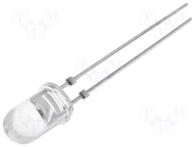
\includegraphics[scale=.5]{IR2.PNG} 
\caption{InfraRed LED }
\end{figure}
\justify There are different types of infrared transmitters depending on their wavelengths, output power and response time.\\
When operated at a supply of 5V, the IR transmitter consumes about 3 to 5 mA of current. \\
IR transmitters can be found in several applications. Some applications require infrared heat and the best infrared source is infrared transmitter. When infrared emitters are used with Quartz, solar cells can be made.
\subsubsection{InfraRed Receiver}
Infrared receivers are also called as infrared sensors as they detect the radiation from an IR transmitter. IR receivers come in the form of photodiodes and phototransistors. Infrared Photodiodes are different from normal photo diodes as they detect only infrared radiation. The picture of a typical IR receiver or a photodiode is shown below.
\begin{figure}[h]
\center
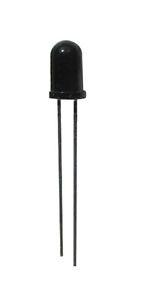
\includegraphics[scale=0.5]{IRR.jpg} 
\caption{IR Receiver }
\end{figure}
\justify Different types of IR receivers exist based on the wavelength, voltage, package, etc. When used in an infrared transmitter – receiver combination, the wavelength of the receiver should match with that of the transmitter.
\subsubsection{Working Principle }
\begin{figure}[h]
\center
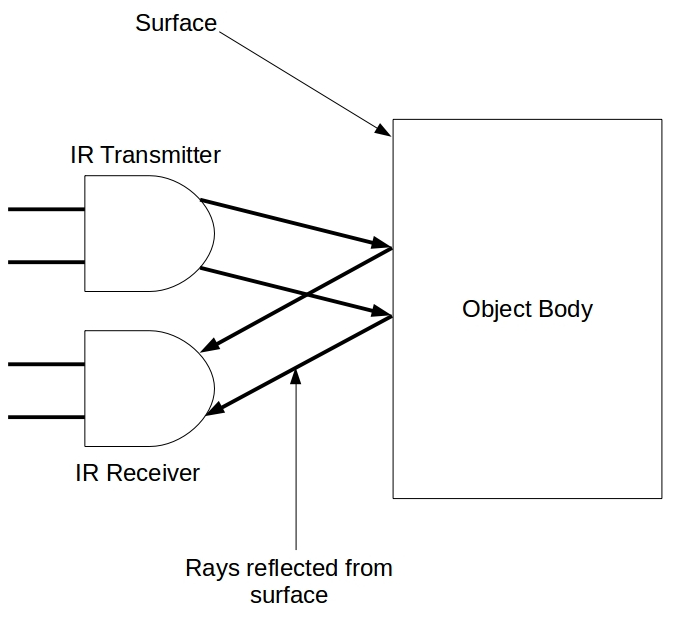
\includegraphics[scale=0.5]{IRpair.jpg} 
\caption{Working Schematic of IR Sensor }
\end{figure}
\justify The principle of an IR sensor working as an Object Detection Sensor can be explained using the following above figure. An IR sensor consists of an IR LED and an IR Photodiode; together they are called as Photo – Coupler or Opto – Coupler.
When the IR transmitter emits radiation, it reaches the object and some of the radiation reflects back to the IR receiver. Based on the intensity of the reception by the IR receiver, the output of the sensor is defined.
\subsubsection{Obstacle Sensing Circuit or IR Sensor Circuit}
A typical IR sensing circuit is shown below.\\
\begin{figure}[h]
\newpage
\center
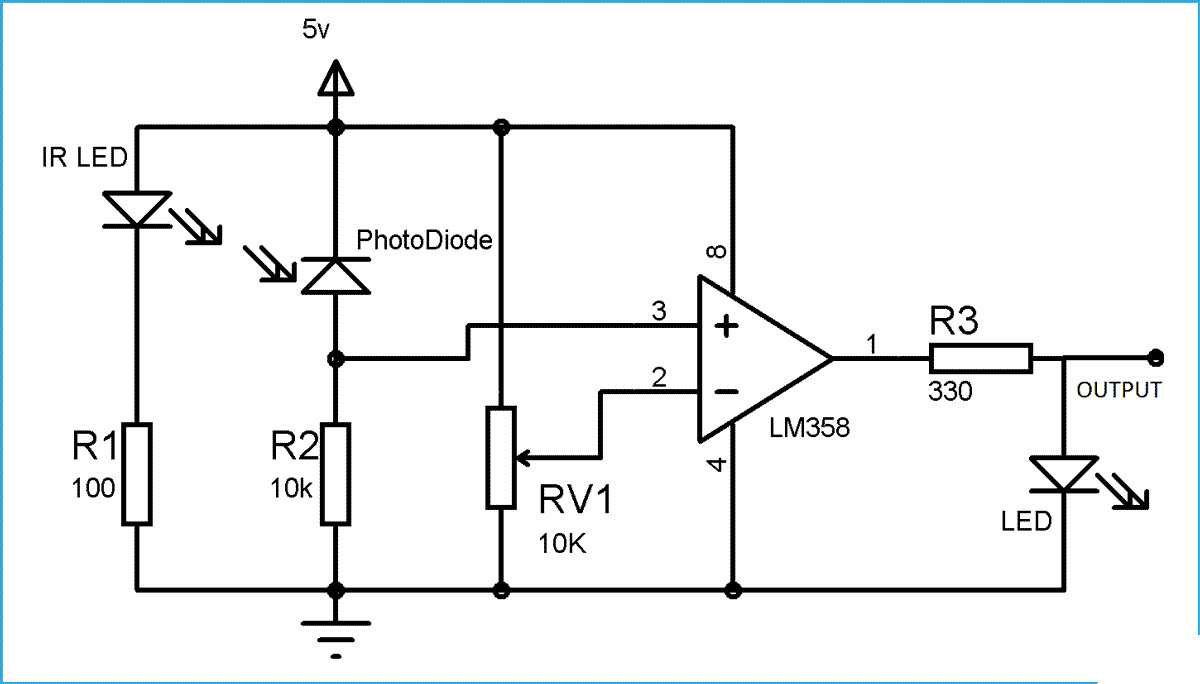
\includegraphics[scale=0.4]{IRsensorcircuit.jpg} 
\caption{IR Sensing circuit Schematic}
\end{figure}
It consists of an IR LED, a photodiode, a potentiometer, an IC Operational amplifier and an LED.\\
IR LED emits infrared light. The Photodiode detects the infrared light. An IC Op – Amp is used as a voltage comparator. The potentiometer is used to calibrate the output of the sensor according to the requirement.\\
When the light emitted by the IR LED is incident on the photodiode after hitting an object, the resistance of the photodiode falls down from a huge value. One of the input of the op – amp is at threshold value set by the potentiometer. The other input to the op-amp is from the photodiode’s series resistor. When the incident radiation is more on the photodiode, the voltage drop across the series resistor will be high. In the IC, both the threshold voltage and the voltage across the series resistor are compared. If the voltage across the resistor series to photodiode is greater than that of the threshold voltage, the output of the IC Op – Amp is high. As the output of the IC is connected to an LED, it lightens up. The threshold voltage can be adjusted by adjusting the potentiometer depending on the environmental conditions.\\
The positioning of the IR LED and the IR Receiver is an important factor. When the IR LED is held directly in front of the IR receiver, this setup is called Direct Incidence. In this case, almost the entire radiation from the IR LED will fall on the IR receiver. Hence there is a line of sight communication between the infrared transmitter and the receiver. If an object falls in this line, it obstructs the radiation from reaching the receiver either by reflecting the radiation or absorbing the radiation.\\
The Infra-Red Sensor module used in the project is the FC-51 Sensor Module\cite{fc51}. It is a Infrared Obstacle Avoidance Proximity Sensor.\\ 
Infrared Obstacle Avoidance Proximity Sensors Module has builtin IR transmitter and IR receiver that sends out IR energy and looks for reflected IR energy to detect presence of any obstacle in front of the sensor module. The module has on board potentiometer that lets user adjust detection range. The sensor has very good and stable response even in ambient light or in complete darkness.\\
The sensor module can be interfaced with Arduino, Raspberry Pi or any microcontroller having IO voltage level of 3.3V to 5V.
\subsection*{Applications}
\begin{enumerate}
\item Obstacle avoidance in robots 
\item Production counting on assembly lines 
\item Presence detection 
\item Security systems 
\end{enumerate}
\subsection*{Features}
\begin{enumerate}
\item LM393 Comparator based detetction circuit is very stable and accurate 
\item On board potentiometer sets obstacle detection range 
\item On board Power LED indicator 
\item On board Obsatcle Detection LED indicator 
\item 3.0MM mounting hole for easy mounting the sensor. 
\item Male header for easy connection 
\item Good Accuracy: By use of Infra-red LED transmitter the module performs well in Ambient light
\end{enumerate}
 \subsection*{Technical Specifications}
\begin{enumerate}
\item  Model Number: FC-51 
\item Detection angle: 35 degree
\item Operating Voltage: 3.0V – 6.0V 
\item Detection range: 2cm – 30cm (Adjustable using potentiometer) 
\item  Overall Dimension: 4.5cm (L) x 1.4 cm (W), 0.7cm (H) 
\item Active output level: Outputs Low logic level when obstacle is detected 
\item In-active output level: Outputs High logic level when obstacle is not detected 
\item Current Consumption: 
\begin{enumerate}
\item at 3.3V : ~23 mA 
	\item at 5.0V: ~43 mA 
\end{enumerate}	
\end{enumerate}
